\documentclass[11pt,a4paper]{article}
\usepackage[margin=2.5cm]{geometry}
\usepackage{amsmath,amssymb,amsthm}
\usepackage{booktabs,array,multirow,longtable}
\usepackage{xcolor}
\usepackage{tcolorbox}
\tcbuselibrary{skins,breakable}
\usepackage{tikz}
\usetikzlibrary{arrows.meta,positioning,shapes.geometric,fit,backgrounds,calc,decorations.pathreplacing}
\usepackage{enumitem}
\usepackage{hyperref}
\usepackage[numbers,sort&compress]{natbib}
\bibliographystyle{unsrtnat}
\hypersetup{colorlinks=true,linkcolor=blue!60!black,urlcolor=blue!60!black,citecolor=green!50!black}
\setlength{\emergencystretch}{2em}

%─── Color palette ───────────────────────────────────────────────────────────
\definecolor{boxblue}{RGB}{220,235,255}
\definecolor{boxorange}{RGB}{255,240,210}
\definecolor{boxgreen}{RGB}{220,245,220}
\definecolor{boxtan}{RGB}{255,245,220}
\definecolor{boxpurple}{RGB}{240,225,255}
\definecolor{boxteal}{RGB}{210,240,238}
\definecolor{boxred}{RGB}{255,230,225}
\definecolor{boxgray}{RGB}{240,240,240}
\definecolor{levzero}{RGB}{245,230,215}
\definecolor{levone}{RGB}{230,240,255}
\definecolor{levtwo}{RGB}{220,240,228}
\definecolor{levthree}{RGB}{250,230,255}
\definecolor{rungmath}{RGB}{210,235,220}
\definecolor{rungcert}{RGB}{255,225,160}
\definecolor{rungphys}{RGB}{190,215,250}

%─── Macros ──────────────────────────────────────────────────────────────────
\newcommand{\term}[1]{\textbf{#1}}
\newcommand{\lean}[1]{\texttt{#1}}
\newcommand{\PHIMDL}{$\Phi_{\rm MDL}$}
\newcommand{\PhiMDL}{\Phi_{\rm MDL}}
\newcommand{\CMCA}{CMCA}
\newcommand{\ZS}{\mathbb{Z}_7}
\newcommand{\poly}{p}
\newcommand{\fMDL}{f_{\rm MDL}}
\newcommand{\CatAL}{\textsc{CatAL}}
\newcommand{\CatAD}{\textsc{CatAD}}
\newcommand{\CatA}{\textsc{CatA}}
\newcommand{\CatB}{\textsc{CatB}}

%─── Title ───────────────────────────────────────────────────────────────────
\title{\textbf{The Levels of the Theory:}\\[6pt]
\large Coarse, Fine, and the Role of the Algebraic Certificate\\[8pt]
\normalsize
\href{https://novaspivack.com/research}{novaspivack.com/research}\quad
\href{https://doi.org/10.5281/zenodo.20560550}{P48 monograph
  (doi.org/10.5281/zenodo.20560550)}\\[4pt]
\normalsize\textit{UGP Physics Tutorial Series}
\\[2pt]\small\href{https://doi.org/\TutorialDOI}{doi.org/\TutorialDOI}}
\author{Nova Spivack}
\newcommand{\TutorialDOI}{10.5281/zenodo.20657872}
\date{2026}

\begin{document}
\setcounter{tocdepth}{2}
\maketitle
\tableofcontents
\newpage

\begin{tcolorbox}[colback=blue!6,colframe=blue!40!black,
  title=\textbf{UGP Physics Tutorial Series}]
\textbf{Prerequisites (read first):} \href{https://doi.org/10.5281/zenodo.20657889}{\emph{The GTE Polynomial: A Step-by-Step
Cheat Sheet}} $\cdot$ \href{https://doi.org/10.5281/zenodo.20657919}{\emph{How the UWCA Works}}
$\cdot$ \href{https://doi.org/10.5281/zenodo.20657885}{\emph{The \boldmath$\Phi_{\rm MDL}$ Field: From Discrete Certificate to
Continuum Physics}}\\[4pt]
\textbf{Next tutorials:} \href{https://doi.org/10.5281/zenodo.20657898}{\emph{How the Standard Model Quantum Numbers Emerge}}
$\cdot$ \href{https://doi.org/10.5281/zenodo.20657870}{\emph{Gravity from Description-Length Minimization}}
$\cdot$ \href{https://doi.org/10.5281/zenodo.20657861}{\emph{The Born Rule as a Theorem}}\\[4pt]
\textbf{See also:} \href{https://doi.org/10.5281/zenodo.20657906}{\emph{The Three-Tape CMCA}} $\cdot$
\href{https://doi.org/10.5281/zenodo.20657895}{\emph{Perfect Self-Containment and MDL}}
\end{tcolorbox}

\begin{tcolorbox}[colback=boxgreen,colframe=green!50!black,
  title=\textbf{Claim-Strength Taxonomy}]
Throughout this tutorial, results are labeled with a confidence grade:
\begin{itemize}[itemsep=2pt]
  \item \textbf{$\mathbf{A}_{\rm Lean}$ (CatAL)} --- Machine-certified in Lean~4 with zero \texttt{sorry} and zero custom axioms.  Independently verifiable by anyone with Lean installed.
  \item \textbf{A/D (CatAD)} --- Analytically derived with full derivation, computationally confirmed.  Not yet machine-certified.
  \item \textbf{A (CatA)} --- Analytically derived; derivation complete but not independently machine-certified.
  \item \textbf{A/D (conditional)} --- Derived under a named, stated premise; the premise is itself an open problem or a CatB assumption.
  \item \textbf{B (CatB)} --- A stated working hypothesis or structural premise; not yet derived.
\end{itemize}
\end{tcolorbox}

%═══════════════════════════════════════════════════════════════════════════════
\section{The Central Puzzle: How Many Layers Does the Theory Have?}
\label{sec:puzzle}
%═══════════════════════════════════════════════════════════════════════════════

\begin{tcolorbox}[colback=boxblue,colframe=blue!40!black,
  title=The question this tutorial answers]
Most physical theories have one layer: the equations of physics describe
what the universe does.
The GTE framework has three or four, depending on how you count.
This tutorial explains what those layers are, why they exist, and what
each one does.
Knowing the layer structure is the key to reading GTE papers
correctly --- especially the level labels (Level~0, Level~1, Level~2,
Level~3) that appear on results throughout the corpus.
\end{tcolorbox}

\bigskip
\noindent
If you have read the \emph{Polynomial Cheat Sheet}~\cite{SpivackTutorialPolynomial} and the \emph{\PHIMDL\ Field} tutorial~\cite{SpivackTutorialPhiMDL},
you already know the two most important facts:
\begin{itemize}[itemsep=4pt]
  \item The GTE polynomial $\poly(L,C,R) = C + R - CR - LCR$ over $\mathrm{GF}(7)$
    is a 19-bit cellular automaton rule --- a discrete algebraic object.
  \item This object is \emph{not the universe}; it is an \term{algebraic certificate}
    for the continuum quantum field $\PhiMDL$, which is what the universe
    is made of.
\end{itemize}
That two-level picture (discrete certificate vs.\ continuum field) captures the
most important distinction.
But the full structure is richer.
The certificate itself comes in multiple layers of increasing concreteness,
from the raw polynomial all the way to the running tape.
And behind the certificate sits a layer of pure arithmetic --- the
mathematical substrate --- that selects and justifies the certificate but
is not itself a physical object.

\medskip
The framework also has a separate organizational vocabulary: the
\term{ontological ladder}, which names the \emph{roles} objects play
(what selects, what certifies, what exists), not just their resolution.
Understanding how the ``levels'' vocabulary and the ``ladder'' vocabulary
relate to each other is the core of this tutorial.

\medskip
The payoff is practical: every result in the GTE paper series is labeled
with its level (\emph{Level~0}, \emph{Level~1}, \emph{Level~2},
\emph{Level~3}, or the coarser \emph{Level~1}/\emph{Level~2}).
Reading those labels correctly tells you how strong a result is, whether
it is a discrete algebraic fact (machine-certifiable in Lean~4) or a
continuum claim (requiring the Lifting Theorem), and whether the claim
depends on any physical interpretation beyond the arithmetic.

%═══════════════════════════════════════════════════════════════════════════════
\section{The Coarse Two-Level Scheme}
\label{sec:coarse}
%═══════════════════════════════════════════════════════════════════════════════

Most GTE papers use a simple two-level vocabulary.
This is the right starting point.

\begin{tcolorbox}[colback=boxorange,colframe=orange!60!black,
  title=The fundamental distinction (coarse two-level scheme)]
\textbf{Level~1 --- The Algebraic Certificate (discrete):}
The CMCA (Chiral Minkowski Cellular Automaton), its PSC-orbit map $\fMDL$,
and the 19-bit polynomial $\poly$.
Discrete, algebraic, machine-certifiable in Lean~4.

\medskip\noindent
\textbf{Level~2 --- The Physical Substrate (continuum):}
$\PhiMDL$ --- the $\ZS$-symmetric Klein-Gordon gauge field on
$\mathbb{R}^{3,1}$.
Continuous, physically real, the actual universe.
\end{tcolorbox}

\subsection{Level~1: The Blueprint}

The Level-1 certificate is the \term{instruction manual} for what the
physical universe must contain.
It is a finite, discrete, algebraic object.
You can run it on a computer.
You can write Lean~4 proofs about it.
You can enumerate its states and verify its behavior exhaustively.

\medskip
\textbf{What the certificate tells you:}
\begin{itemize}[itemsep=5pt]
  \item \textbf{Which particle types must exist.}
    Exactly five $\ZS$ winding sectors pass the PSC filter:
    $\{0,2,3,4,6\}$, corresponding to the SM particle classes
    (\lean{psc\_admissible\_sectors}, zero sorry).

  \item \textbf{Why there are exactly three generations.}
    The $\ZS^5$ orbit under $\fMDL$ has exactly three non-vacuum
    orbit types, cycling with period 3.
    This is a consequence of the $\ZS$ arithmetic, not an external input.
    Machine-certified: \lean{three\_generations\_physical} (zero sorry).

  \item \textbf{The electric charge formula.}
    $Q = w_{\rm c}/3$, where $w_{\rm c}$ is the centered representative of the
    $\ZS$ winding number.
    Machine-certified: \lean{gte\_charge\_is\_linear\_projection} (zero sorry).

  \item \textbf{Topological structure and conservation laws.}
    Winding-number conservation at every interaction vertex;
    color confinement; $\theta_{\rm QCD} = 0$ by three independent
    algebraic proofs.

  \item \textbf{Computational universality.}
    The binary restriction of $\poly$ is Rule~110, the unique CA rule with
    a machine-certified proof of Turing universality.
\end{itemize}

All of these facts live at Level~1: they are algebraic facts about the discrete
certificate, provable without any reference to the continuum field.

\subsection{Level~2: The Building}

Level~2 is $\PhiMDL$ --- the $\ZS$-symmetric Klein-Gordon gauge field with
internal symmetry group $F_{21} = \ZS\rtimes\mathbb{Z}_3$, evolving on
$\mathbb{R}^{3,1}$.

\medskip
This is what the universe \emph{is}.
Elementary particles are BPS (Bogomolny-Prasad-Sommerfield) topological
kink solitons of this field, classified by their $\ZS$ winding number.
Spacetime, quantum mechanics, and all cosmological observables emerge from
its dynamics.

\medskip
\textbf{What Level~2 adds beyond Level~1:}
\begin{itemize}[itemsep=4pt]
  \item Exact Lorentz invariance (any finite-resolution CA has a preferred
    frame; the continuum field does not).
  \item Exact particle masses (derived via the orbit cascade and the
    Self-Referential Renormalization Group; see the \emph{Masses} tutorial~\cite{SpivackTutorialMasses}).
  \item Spacetime geometry (3+1D Minkowski spacetime, General Relativity).
  \item Full quantum field theory (Hilbert space structure, scattering
    amplitudes).
\end{itemize}

\subsection{A Table: What Lives at Each Level}

\bigskip
\begin{center}
\begin{tabular}{@{}p{5.5cm}cc@{}}
\toprule
\textbf{Result / claim} & \textbf{Coarse Level} & \textbf{Cert} \\
\midrule
Three SM generations exist & Level~1 & \CatAL \\
Electric charge formula $Q = w_{\rm c}/3$ & Level~1 & \CatAL \\
Strong CP angle $\theta = 0$ & Level~1 & \CatAL \\
Color confinement & Level~1 & \CatAL \\
Quantum numbers of all SM fermions & Level~1 & \CatAL \\
Winding-sector admissibility ($\{0,2,3,4,6\}$) & Level~1 & \CatAL \\
Fermion / boson statistics & Level~1 & \CatAL \\
Turing universality (Rule~110 link) & Level~1 & \CatAL \\
\midrule
Exact Lorentz invariance & Level~2 & \CatAL \\
Particle masses & Level~2 & \CatAD \\
3+1 spacetime dimensions & Level~2 & \CatAL \\
Einstein equations $G_{\mu\nu} = 8\pi G\,T_{\mu\nu}$ & Level~2 & \CatAD \\
Newton's constant $G_N$ & Level~2 & \CatAD \\
Born rule & Level~2 & \CatAL \\
Cosmological constant bracket & Level~2 & \CatAD \\
\bottomrule
\end{tabular}
\end{center}
\bigskip

\noindent
The coarse scheme works well for most purposes.
Whenever a paper says ``Level~1 certificate'' or ``Level~2 field,''
it means the CA/algebraic side or the continuum/physical side.

%═══════════════════════════════════════════════════════════════════════════════
\section{The Fine-Grained Four-Level Scheme}
\label{sec:fine}
%═══════════════════════════════════════════════════════════════════════════════

For detailed derivations --- especially when tracking exactly which structural
features come from where --- a finer vocabulary breaks the ``Level~1 certificate''
into three sub-levels.

\begin{tcolorbox}[colback=boxblue,colframe=blue!40!black,
  title={The GTE Computational Architecture: One System, Four Levels},
  breakable]
\small
The polynomial $\poly(L,C,R) = C+R-CR-LCR$ defines a single physical system
expressed at four levels of description; each level is the same physics at a
different scale of resolution.

\medskip
\noindent\textbf{Level~0 --- Raw Polynomial} (\emph{Object~0}).
The $k{=}7$, $r{=}1$ CA rule over $\mathrm{GF}(7)$, as a mathematical object.
Class-3 chaotic on generic $\ZS$ inputs; Class-4 (Rule~110) on $\{0,1\}$-inputs.
MDL $+$ PSC select it uniquely from $7^{343}$ candidates
(\lean{mdl\_ca\_rule\_coding\_closed}, \CatAL).
No dynamics yet; just the formula.

\medskip
\noindent\textbf{Level~1 --- PSC-Projected Orbit Map} (\emph{Object~1}, $\fMDL$).
The restriction of $\poly$ to PSC-admissible inputs.
$\fMDL$ maps 14 of the 343 neighborhoods non-trivially; all others produce the
vacuum.
On the isolated 5-cell ring, $\fMDL$ runs the SM generation orbit
$\mathrm{GEN}_1\to\mathrm{GEN}_2\to\mathrm{GEN}_3\to\mathrm{VAC}$ (\CatAL).
This is the abstract discrete dynamics --- orbit structure, quantum numbers,
generation count.

\medskip
\noindent\textbf{Level~2 --- CMCA Tape}.
$\fMDL$ embedded in a 1D spatial tape with a chiral pair
(Rule~110 forward / Rule~124 backward) and an inner $\tau_c$
first-passage clock gating outer updates asynchronously.
This is the CMCA: a running, spatially-extended cellular automaton.
Three tapes sharing a global outer clock $\tau_c^{\rm out}$ give the
$3{+}1$D architecture (Dimensional Protocol Principle, \CatAL).

\medskip
\noindent\textbf{Level~3 --- Continuum Field} (\emph{Object~2}, $\PhiMDL$).
The Algebraic Lifting Theorem (\lean{algebraic\_lifting\_theorem}, \CatAL) maps
the CMCA's discrete structure to the $\ZS$-symmetric Klein-Gordon field $\PhiMDL$.
SM particles are BPS kink solitons; all SM parameters, spacetime, QM,
and cosmology emerge at this level.

\medskip
\noindent\textit{Relation to the coarse two-level scheme:}
Levels~0--2 collectively constitute the \emph{algebraic certificate} ---
``Level~1'' in the coarse scheme.
Level~3 here is the \emph{continuum physical substrate} --- ``Level~2'' in
that framework.
The four-level description is a finer-grained view; both schemes are valid.
\end{tcolorbox}

\subsection{Plain-English Guide to Each Fine Level}

\begin{tcolorbox}[colback=levzero,colframe=orange!50!black,
  title=Level 0 --- The Raw Polynomial]
\textbf{What it is:} Just the formula $\poly(L,C,R) = C + R - CR - LCR$
over $\mathrm{GF}(7)$, as a mathematical expression.
No spacetime, no dynamics, no orbit --- just the arithmetic rule.

\medskip\noindent
\textbf{What you can prove here:}
Algebraic identities; the coefficient structure; the link to Rule~110
(when restricted to $\{0,1\}$ inputs); MDL minimality within the
multilinear polynomial class; the fact that exactly four monomials are
needed.

\medskip\noindent
\textbf{Plain English:}
Level~0 is the recipe card, before you've cooked anything.
\end{tcolorbox}

\begin{tcolorbox}[colback=levone,colframe=blue!50!black,
  title=Level 1 --- The PSC-Projected Orbit Map ($f_{\rm MDL}$)]
\textbf{What it is:} The polynomial restricted to the PSC-admissible
neighborhood configurations.
$\fMDL$ turns the abstract rule into a dynamics on the 5-cell ring that
generates the Standard Model generation orbit.

\medskip\noindent
\textbf{What you can prove here:}
Three-generation structure; Garden-of-Eden stability of gen$_1$;
winding-sector admissibility; charge quantization;
fermion/boson statistics from group order;
color confinement as MDL-inadmissibility of free colored states;
$\theta_{\rm QCD} = 0$.

\medskip\noindent
\textbf{Plain English:}
Level~1 is the first time the recipe actually tells you something about
the finished dish: what ingredients must appear, in what combinations.
\end{tcolorbox}

\begin{tcolorbox}[colback=levtwo,colframe=green!50!black,
  title=Level 2 --- The CMCA Tape]
\textbf{What it is:} The orbit map embedded in a running, spatially-extended
automaton --- the Chiral Minkowski Cellular Automaton.
The tape has the full chiral architecture (Rule~110 + Rule~124) and the
inner $\tau_c$ first-passage clock.
Three tapes sharing a clock give 3+1D.

\medskip\noindent
\textbf{What you can prove here:}
Dimensional Protocol Principle (DPP); 3+1D Minkowski structure;
SR time dilation; Lorentz algebra $\mathfrak{so}(1,3)$;
holographic area scaling;
kink-spectrum existence (via the Lifting Theorem).

\medskip\noindent
\textbf{Plain English:}
Level~2 is the kitchen --- the full apparatus running.
The dish is being cooked, but it is not yet the physical meal.
\end{tcolorbox}

\begin{tcolorbox}[colback=levthree,colframe=purple!50!black,
  title=Level 3 --- The Continuum Field ($\Phi_{\rm MDL}$)]
\textbf{What it is:} The unique continuum Lorentz-invariant quantum field
whose algebraic structure is certified by Levels~0--2.
$\PhiMDL$ is a $\ZS$-symmetric Klein-Gordon gauge field on $\mathbb{R}^{3,1}$
with exact symmetry group $F_{21} = \ZS\rtimes\mathbb{Z}_3$.
Particles are its BPS kink solitons.

\medskip\noindent
\textbf{What you can prove here:}
Exact Lorentz invariance; particle masses; spacetime geometry; gravity;
quantum mechanics; cosmological observables.

\medskip\noindent
\textbf{Plain English:}
Level~3 is the finished building.
This is what exists.
\end{tcolorbox}

\subsection{A Table: Fine-Level Scheme}

\bigskip
\begin{center}
\begin{tabular}{@{}clp{6.2cm}l@{}}
\toprule
\textbf{Fine Level} & \textbf{Name} & \textbf{Key results} & \textbf{Coarse} \\
\midrule
0 & Raw polynomial $\poly$ & MDL minimality; polynomial form; Rule~110 link & L1 cert \\
1 & $\fMDL$ orbit map & Quantum numbers; 3 generations; color confinement & L1 cert \\
2 & CMCA tape & 3+1D; SR; holography; DPP & L1 cert \\
3 & $\PhiMDL$ field & Masses; GR; QM; cosmology & L2 substrate \\
\bottomrule
\end{tabular}
\end{center}
\bigskip

\begin{tcolorbox}[colback=boxgray,colframe=gray!50!black,
  title=When to use which scheme]
\textbf{Use the coarse (two-level) scheme} when:
\begin{itemize}[itemsep=2pt]
  \item You are discussing a result in a paper.
  \item You need to decide: ``is this a machine-certifiable algebraic fact, or
    does it depend on the continuum field?''
  \item You are reading claims boxes (orange colorboxes in GTE papers).
\end{itemize}

\medskip\noindent
\textbf{Use the fine (four-level) scheme} when:
\begin{itemize}[itemsep=2pt]
  \item You need to know whether a result depends on the polynomial's
    structure alone (Level~0), the orbit dynamics (Level~1), the
    full spatiotemporal tape (Level~2), or the continuum limit (Level~3).
  \item You are tracing which step in a derivation introduces the
    first spacetime structure.
  \item You are reading P41 (CMCA), P45 (three-tape CMCA), or
    the Mathematical Substrate chapter of P48~\cite{SpivackGTECompleteFramework}.
\end{itemize}
\end{tcolorbox}

%═══════════════════════════════════════════════════════════════════════════════
\section{The Ontological Ladder}
\label{sec:ladder}
%═══════════════════════════════════════════════════════════════════════════════

The levels grade \emph{resolution} of description.
The ontological ladder grades \emph{role}.
These are two orthogonal ways of organizing the same framework.

\begin{tcolorbox}[colback=boxgreen,colframe=green!50!black,
  title=The Ontological Ladder (canonical definition from P48 Chapter~4)]
The theory's objects occupy three rungs, and the rungs must not be conflated.

\medskip\noindent
\textbf{Rung~1 --- Mathematical Substrate.}
The UGP/GTE arithmetic: the ridge sieve, the integer triples $(a,b,c;\,g)$
and map $T$, the generation orbit, and the UWCA evaluator.
Pure number theory and combinatorics, prior to any physical interpretation.
It is the domain in which both of MDL's selections operate: the seed
selection (the Lepton Seed $(1, 73, 823)$) and the rule selection
(the polynomial $\poly$).
\emph{Not a physical object.}
Its role is: \textbf{to select}.

\medskip\noindent
\textbf{Rung~2 --- Algebraic Certificate.}
What those selections produce: the 19-bit polynomial $\poly$,
its PSC-orbit map $\fMDL$, and the CMCA tape
(fine Levels~0--2 of the four-level architecture).
Machine-checkable in Lean~4.
\emph{Not a physical object.}
Its role is: \textbf{to certify}.

\medskip\noindent
\textbf{Rung~3 --- Physical Substrate.}
$\PhiMDL$: the $\ZS$-symmetric Klein-Gordon gauge field on
$\mathbb{R}^{3,1}$.
\emph{The only rung that physically exists.}
Its role is: \textbf{to be}.
\end{tcolorbox}

\subsection{Rung~1: The Mathematical Substrate}

The mathematical substrate is the number-theoretic ground in which the
framework lives before any physical claim is made.

\medskip
The \term{ridge sieve} filters which integer triples are arithmetically
coherent.
At ridge level $n = 10$ (forced by four independent arithmetic certificates),
exactly six triples survive; the Minimum Description Length principle selects
the unique lexicographically minimal survivor: the Lepton Seed
$(1, 73, 823)$.

\medskip
Applying the GTE map $T$ twice to the Lepton Seed produces the three
$N_{\rm eff}$ values 73, 42, 275 --- the electron, muon, and tau
informational addresses.
This three-generation cascade is pure arithmetic: no physics postulated,
no parameters chosen.

\medskip
The \term{Universal Windowed Cellular Automaton (UWCA)} is the mathematical
substrate's native computer --- a finite-local evaluator on which Rule~110
demonstrably runs.
Its existence shows that the arithmetic is \emph{self-describing}: the same
substrate that produces the generation orbit also supports the computation
needed to check it.

\medskip
\textbf{The key point:} the mathematical substrate does not have a ``level''
in the four-level scheme.
The level vocabulary starts at Level~0 (the polynomial), which is already
the \emph{output} of the substrate's MDL selection.
The substrate is below the bottom of the level ladder.

\subsection{Rung~2: The Certificate}

The certificate is what the mathematical substrate's MDL selections produce.
It spans fine Levels~0--2: the polynomial (Level~0), the orbit map (Level~1),
and the running tape (Level~2).

\medskip
The certificate is not an approximation to the physical field.
It is the \emph{proof system} that certifies what the physical field must
contain.
Run the certificate on a computer and you are running a mechanically
verifiable proof about the structure of matter.

\medskip
\textbf{An important subtlety:} there is a sense in which the certificate is
``closer to'' the physical field than the mathematical substrate is --- the
certificate already contains all the algebraic structure of Standard Model
physics --- but it is not the physical field.
The Lorentz invariance that the physical universe exhibits exactly cannot be
achieved by any finite-resolution CA (this is the No-CA-Replica Theorem;
see \S\ref{sec:noca}).

\subsection{Rung~3: The Physical Substrate}

The physical substrate is $\PhiMDL$.
It is the only rung that physically exists: the actual quantum field pervading
$\mathbb{R}^{3,1}$, whose topological kink excitations are the elementary
particles of the Standard Model.

\medskip
$\PhiMDL$ has \emph{exact} Lorentz invariance, which requires the
continuum limit $M \to \infty$.
It has exact particle masses, exact scattering amplitudes, exact spacetime
geometry.

\begin{tcolorbox}[colback=boxblue,colframe=blue!40!black,
  title=The ladder is orthogonal to the level vocabulary]
The four fine levels (0--3) and the three ontological rungs are two
different ways of talking about the same framework.

\begin{itemize}[itemsep=4pt]
  \item \textbf{Levels} ask: \emph{how coarsely are we describing the system?}
    (Raw rule? Orbit? Running tape? Continuum limit?)
  \item \textbf{Rungs} ask: \emph{what role does this object play?}
    (Selector? Certifier? The thing that exists?)
\end{itemize}

Levels~0--2 all sit on Rung~2 (certificate).
Level~3 sits on Rung~3 (physical substrate).
Rung~1 (mathematical substrate) sits below the level vocabulary entirely.
\end{tcolorbox}

\subsection{The Two Key Transitions on the Ladder}

\medskip
\noindent\textbf{Rung~1 $\to$ Rung~2: MDL Selection.}
The mathematical substrate does not automatically produce the certificate.
Two selections are required, both governed by the MDL principle:
\begin{enumerate}[itemsep=3pt]
  \item \emph{Seed selection:} MDL selects the Lepton Seed $(1, 73, 823)$
    from the ridge sieve survivors
    (\lean{rsuc\_theorem}, \lean{mdl\_selects\_LeptonSeed}, \CatAL).
  \item \emph{Rule selection:} MDL, applied to the generation orbit's
    parity shadow, selects the unique polynomial $\poly$
    (\lean{mdl\_ca\_rule\_coding\_closed}, \CatAL).
\end{enumerate}

The two selections compose sequentially: the seed selection produces the
orbit, and the orbit's parity shadow drives the rule selection.
The two arms of the framework (the particle \emph{spectrum}, from the orbit;
and the particle \emph{dynamics}, from the polynomial) both trace back to
one arithmetic substrate and two MDL applications.

\medskip\noindent
\textbf{Rung~2 $\to$ Rung~3: The Algebraic Lifting Theorem.}
This transition is covered in detail in \S\ref{sec:lifting}.
The Lifting Theorem is the certified bridge that guarantees: every algebraic
fact proved in the certificate holds in the physical field.

%═══════════════════════════════════════════════════════════════════════════════
\section{What the Certificate Does --- and Does Not Do}
\label{sec:cert}
%═══════════════════════════════════════════════════════════════════════════════

\subsection{What the Certificate Certifies}

The certificate certifies everything that is a discrete algebraic fact
about the universe's structure:

\begin{itemize}[itemsep=5pt]
  \item Which topological excitations are PSC-admissible (i.e., which
    particle types must exist).
  \item What quantum numbers they carry ($\ZS$ winding number,
    $\mathbb{Z}_3$ color charge, generation index).
  \item Conservation laws at every interaction vertex.
  \item Color confinement (free colored quarks are PSC-inadmissible:
    displaying an isolated colored state costs extra MDL bits).
  \item The strong CP angle $\theta_{\rm QCD} = 0$ by three independent
    algebraic proofs from $F_{21}$ group theory.
  \item Turing universality (the binary restriction is Rule~110;
    any computation can be simulated).
  \item 3+1D Minkowski structure via the Dimensional Protocol Principle.
\end{itemize}

All of these facts hold at \emph{every} lattice resolution $M \geq 1$.
They do not depend on the continuum limit.
This is the content of the Algebraic Descent Theorem (\S\ref{sec:descent}).

\subsection{What the Certificate Cannot Certify}
\label{sec:cert_cannot}

\begin{tcolorbox}[colback=boxteal,colframe=teal!50!black,
  title=What Level~1 cannot certify (directly)]
\begin{itemize}[itemsep=4pt]
  \item \textbf{Exact Lorentz invariance.}
    Any finite-resolution CA has a preferred frame.
    For a CA with $M$ cells per unit length, the Nyquist residual
    $\varepsilon_0(M) = \pi^2/(3M^2)$ is strictly positive for all finite $M$.
    Exact Lorentz invariance requires $M \to \infty$, which is $\PhiMDL$.

  \item \textbf{Exact particle masses.}
    Masses come from the Level-3 orbit cascade (energy of the $\PhiMDL$ kinks)
    and the SRRG bridge, not from the CA's discrete rule.
    The CA certifies \emph{which particles exist}; the continuum field gives
    their masses.

  \item \textbf{Specific spacetime microstructure at Compton scale.}
    The Lifting Theorem certifies existence of a particle with given quantum
    numbers, but does not identify which specific CA glider pattern
    corresponds to the electron at Compton scale.
    That identification is an open problem.
\end{itemize}
These properties require the continuum field $\PhiMDL$.
\end{tcolorbox}

\subsection{The No-CA-Replica Theorem}
\label{sec:noca}

Why can't the universe simply be the cellular automaton?
The answer is Lorentz invariance --- and it is a theorem, not merely a
philosophical preference.

\begin{tcolorbox}[colback=boxred,colframe=red!50!black,
  title={Theorem: No-CA-Replica (\CatAL, zero sorry)}]
For every finite lattice resolution $M > 0$:
\[
  \varepsilon_0(M) \;=\; \frac{\pi^2}{3M^2} \;>\; 0.
\]
No finite-resolution discrete model can achieve exact Lorentz invariance.
The continuum limit $M \to \infty$ is the unique exact Lorentz-invariant
model in the $\ZS$ class, and that limit is $\PhiMDL$.

\smallskip\noindent
\textbf{Lean cert:} \lean{no\_finite\_ca\_exact\_lorentz\_replica}
(zero sorry, \lean{CMCAContinuumLimit.lean}, ugp-lean).
\end{tcolorbox}

\medskip\noindent
\textbf{Plain-English meaning:}
Any finite cellular automaton has a \emph{lattice}: a preferred grid of
cells.
That grid defines a preferred frame --- the frame in which the grid is at
rest.
At high velocities, Lorentz boosts make the lattice structure visible,
breaking the symmetry of special relativity.
The bigger the lattice cells (smaller $M$), the bigger the violation.
At $M = 7$ (the natural scale for the CA), the error is $\sim 6.7\%$.
The \emph{only} CA with zero error is the one with infinitely fine cells ---
which is the continuum field $\PhiMDL$.

\medskip
\textbf{What the theorem does NOT say:}
It does not say the CA is wrong or useless.
It says the CA is the wrong \emph{kind} of object to be the physical
substrate.
The CA is a certificate --- a proof engine.
A proof engine does not need to be the physical universe; it needs to be
correct about what the physical universe must contain.
The CA at $M = 7$ certifies algebraic facts (charge quantization,
three generations, $\theta = 0$, \ldots) with \emph{zero} error.
The $6.7\%$ error applies only to geometrical/Lorentz-invariance properties,
not to the algebraic facts.

\begin{tcolorbox}[colback=boxblue,colframe=blue!40!black,
  title=The blueprint is not wrong; it is not a building]
The no-CA-replica theorem does not mean the CMCA is incorrect.
It means the CMCA is the wrong \emph{kind} of object to be the physical
substrate.
The blueprint of a building is not wrong about what the building contains
--- it just is not made of steel and glass.
\end{tcolorbox}

%═══════════════════════════════════════════════════════════════════════════════
\section{The Algebraic Lifting Theorem}
\label{sec:lifting}
%═══════════════════════════════════════════════════════════════════════════════

\begin{tcolorbox}[colback=boxgreen,colframe=green!50!black,
  title={Theorem: Algebraic Lifting (\CatAL, zero sorry, zero custom axioms)}]
Let $B$ be a PSC-admissible beable with positive dynamical weight.
Then $B$ determines a physical observable at the Compton scale carrying the
same $\ZS$ winding number, $\mathbb{Z}_3$ color charge, and generation index
as $B$.
In particular: charge quantization, color structure, the three-generation
hierarchy, and $S$-matrix quantum numbers proved at the beable level hold
at the physically observable Compton scale.

\smallskip\noindent
\textbf{Lean cert:}
\lean{algebraic\_lifting\_theorem}
(\lean{LiftingTheorem.lean}, ugp-lean, zero sorry, zero custom axioms).
\end{tcolorbox}

\subsection{What ``Lifting'' Means}

\term{Lifting} is the process of taking a result proved in the discrete
certificate (Level~1, the CA) and concluding that the corresponding statement
holds in the continuum field (Level~2/3, $\PhiMDL$).

\medskip
A useful analogy from mathematics: completeness theorems in logic.
In formal logic, a theory is \emph{complete} if every statement true in
the intended model is provable from the axioms.
The Lifting Theorem plays an analogous role: every algebraic fact proved in
the CMCA (the discrete model) holds in $\PhiMDL$ (the physical realization).
The CA is the model; $\PhiMDL$ is the full theory.

\medskip
More concretely: suppose you prove in the CA that winding number is conserved
at every interaction vertex.
The Lifting Theorem guarantees that winding number is also conserved at every
interaction vertex in $\PhiMDL$.
The proof happens in the CA (where it is a finite computation, machine-checkable);
the conclusion holds in the physical universe.

\subsection{What Can Be Lifted vs.\ What Cannot}

\begin{itemize}[itemsep=5pt]
  \item \textbf{Can be lifted:} any property in the $F_{21} = \ZS\rtimes\mathbb{Z}_3$
    winding sector --- quantum numbers, conservation laws, topological charges,
    generation structure, admissibility conditions, color charges.
  \item \textbf{Cannot be lifted directly:} geometrical properties
    (Lorentz invariance, scattering amplitudes at high momentum) that
    depend on the continuum limit.
    These are not \emph{forbidden} --- they are established by the no-CA-replica
    theorem and the $\PhiMDL$ Lagrangian, not by the Lifting Theorem.
\end{itemize}

\subsection{A Worked Example: The Three Vacua and Color Charges}

The $\PhiMDL$ potential has seven degenerate minima (vacua) at
$\Phi_k = 2\pi k/7$ for $k \in \{0, 1, \ldots, 6\}$.
The three \term{ground states} of the CA are $\{0, 1, 5\}$ --- the three
fixed points of the polynomial under iteration.

\medskip
At Level~0 (raw polynomial), this is a pure algebraic fact about the
fixed points of $\poly$.
Via the Lifting Theorem, this translates to the three \emph{color charges}
of QCD: there are exactly three color states because the CA has exactly
three ground states.
The algebraic structure at Level~0 lifts to the physical gauge structure at
Level~3.

\medskip
\textbf{Another example:} the electron.

\medskip
\begin{center}
\begin{tabular}{@{}p{6.0cm}l@{}}
\toprule
\textbf{Level~1 (certificate says)} & \textbf{Level~3 (physics says)} \\
\midrule
Beable $[1,5,2,2,1]$ with winding $W = 4$, & $w=4$ kink in $\PhiMDL$,\quad $Q = -1$, \\
Garden-of-Eden (no predecessors), & $J = 1/2$, \quad $m_e = 0.511$\,MeV \\
fermionic statistics (ord$(4) = 3$ in $\ZS^*$) & \\
\bottomrule
\end{tabular}
\end{center}

\medskip\noindent
The charge, statistics, and generation stability all follow from Level~1
arithmetic.
The mass and the spin assignment follow from the Lifting Theorem
combined with the continuum kink spectrum.
Neither the charge nor the mass is a free parameter.

\subsection{Why the Lifting Theorem Makes Machine-Certified Physics Possible}

Before the Lifting Theorem, there would be a gap: you could prove things
about the CA, but those proofs would be about an abstract discrete object,
not about the physical universe.
The Lifting Theorem closes that gap.

\medskip
Once the Lifting Theorem is in hand, a Lean~4 proof that certifies some
algebraic property of the CA \emph{is} a proof about particle physics.
This is why GTE papers can state results like:
``The electron's charge is $-1$ (zero sorry, zero custom axioms).''
The proof runs in a finite discrete computer, about a finite discrete object;
the Lifting Theorem guarantees the conclusion holds in the physical universe.

%═══════════════════════════════════════════════════════════════════════════════
\section{The Algebraic Descent Theorem}
\label{sec:descent}
%═══════════════════════════════════════════════════════════════════════════════

\begin{tcolorbox}[colback=boxblue,colframe=blue!40!black,
  title={Theorem: Algebraic Descent (\CatAL, zero sorry)}]
Every $F_{21} = \ZS\rtimes\mathbb{Z}_3$ conservation law,
charge quantization condition, and generation structure certified at the
discrete CMCA level holds in any continuum realization at any lattice
resolution $M \geq 1$.

Charge quantization, color confinement, asymptotic freedom ($b_0 = 7$),
and the strong-CP resolution $\theta_{\rm QCD} = 0$ are $M$-independent.
Only geometric properties (Lorentz invariance, SR accuracy) require
$M \to \infty$.

\smallskip\noindent
\textbf{Lean cert:}
\lean{algebraic\_descent\_theorem}
(\lean{AlgebraicDescentTheorem.lean}, ugp-lean, zero sorry).
\end{tcolorbox}

\subsection{The Other Direction}

The Descent Theorem is the converse of the Lifting Theorem.
Where Lifting says ``certificate $\Rightarrow$ physics,'' Descent says
``physics $\Rightarrow$ certificate.''

\medskip
More precisely: any physical model that respects the $F_{21}$ winding algebra
\emph{must also} enforce all the discrete Level-1 constraints.
The continuum field cannot escape what the CA forbids.

\medskip
This has a striking practical consequence.
The Descent Theorem is why all the algebraic structure certified in the CA
holds for $\PhiMDL$ at \emph{every} scale, not just in the continuum limit.
Even at $M = 7$ (one cell per lattice unit), the charge quantization,
three-generation structure, and color confinement constraints are exact ---
no approximation is involved.

\subsection{Why the Descent Theorem Matters for Lean Certification}

The Descent Theorem explains why Lean~4 can certify physical predictions.

\begin{itemize}[itemsep=5pt]
  \item The certification \emph{happens} at Level~1 (the CA is checkable;
    it is a finite discrete object).
  \item The Lifting Theorem says: the certificate implies the physics.
  \item The Descent Theorem says: the physics must respect the certificate.
  \item Together: the CA and $\PhiMDL$ are algebraically equivalent in the
    SM winding sector --- two descriptions of the same object at different
    scales, related by a certified bidirectional correspondence.
\end{itemize}

\subsection{A Worked Example: Color Confinement}

Consider the statement: ``An isolated quark cannot be observed as a free
particle.''

\medskip
\noindent
\textbf{In the CA (Level~1):}
A free quark would carry winding $w \in \{2, 6\}$.
Displaying such a state requires an extra $\log_2 9 \approx 3.17$ MDL bits
to specify its color.
MDL minimality forbids this: isolated colored states are PSC-inadmissible.
Machine-certified: \lean{psc\_forbids\_free\_colored\_quarks} (zero sorry).

\medskip
\noindent
\textbf{By Descent to $\PhiMDL$:}
The Descent Theorem guarantees that the PSC-inadmissibility established at
Level~1 holds at every resolution $M \geq 1$, including the continuum.
$\PhiMDL$ therefore also forbids free colored quarks: color confinement is
an exact algebraic fact of the continuum theory, certified by the CA.

\medskip
\noindent
\textbf{What this means:}
A 19-bit polynomial over a 7-element finite field certifies --- with zero
sorry and zero free parameters --- that quark confinement holds in the
physical universe.

%═══════════════════════════════════════════════════════════════════════════════
\section{Level Framing in Practice: How GTE Papers Use These Labels}
\label{sec:practice}
%═══════════════════════════════════════════════════════════════════════════════

\subsection{Why Level Labels Matter}

Every result in the GTE corpus carries a level label.
This is not decoration --- it is a precision commitment.
A Level~0 algebraic fact (a property of the raw polynomial) is maximally
strong: it follows from pure arithmetic and can be verified by exhaustive
enumeration if needed.
A Level~3 claim (about $\PhiMDL$) may require additional continuum
assumptions and the Lifting Theorem.

\medskip
Knowing the level tells you:
\begin{enumerate}[itemsep=4pt]
  \item \textbf{How checkable the claim is.}
    Level~0--2 claims are in principle machine-verifiable in Lean~4.
    Level~3 claims require the Lifting Theorem and sometimes additional
    continuum physics arguments.

  \item \textbf{What the claim depends on.}
    A Level~0 claim depends only on the polynomial's arithmetic.
    A Level~3 claim additionally depends on the continuum field structure
    and the bridge theorems.

  \item \textbf{How to cite it honestly.}
    Writing ``\textsc{CatAL}'' next to a Level~0/1 result tells the reader
    it is Lean-certified.
    Writing ``\textsc{CatAD}'' next to a Level~3 result tells the reader it
    is analytically derived and computationally confirmed, but the full
    machine proof runs through the Lifting Theorem.
\end{enumerate}

\subsection{Worked Examples of Level Framing}

\medskip
\begin{tcolorbox}[colback=levzero,colframe=orange!50!black,
  title={Level~0 example: ground states are $\{0,1,5\}$}]
\textbf{Claim:} The fixed points of $\poly(x,x,x)$ over $\mathrm{GF}(7)$
are exactly $\{0, 1, 5\}$.

\textbf{Level:} 0 (raw polynomial arithmetic).

\textbf{Why level 0:} This is a statement about the formula
$\poly(x,x,x) = x$ over $\mathrm{GF}(7)$.
No orbit, no tape, no continuum.
Checkable by evaluating seven numbers.

\textbf{Cert:} \CatAL\ (decidable by exhaustive enumeration; zero sorry).
\end{tcolorbox}

\begin{tcolorbox}[colback=levone,colframe=blue!50!black,
  title={Level~1 example: strong CP angle $\theta_{\rm QCD} = 0$}]
\textbf{Claim:} The strong CP angle $\theta_{\rm QCD} = 0$ exactly.

\textbf{Level:} 1 (group theory of $\fMDL$ and $F_{21}$).

\textbf{Why level 1:} Three independent algebraic proofs from the
$F_{21} = \ZS\rtimes\mathbb{Z}_3$ group structure establish this ---
no continuum field theory required.
The argument uses the orbit map and its symmetry properties.

\textbf{Cert:} \CatAL\ (three independent machine-certified proofs; zero sorry).
\end{tcolorbox}

\begin{tcolorbox}[colback=levtwo,colframe=green!50!black,
  title=Level~2 example: 3+1D Minkowski structure]
\textbf{Claim:} Three CMCA tapes sharing a common outer clock produce
$3{+}1$D Minkowski spacetime.

\textbf{Level:} 2 (CMCA tape architecture --- the Dimensional Protocol
Principle).

\textbf{Why level 2:} The claim is about three running tapes sharing
a clock, and whether their tensor product gives the correct spacetime.
The tape is the Level-2 object; the DPP is a Level-2 theorem.

\textbf{Cert:} \CatAL\
(\lean{dimensional\_protocol\_principle\_master},
\lean{cmca\_tensor\_product\_gives\_31d\_minkowski};
zero sorry; ugp-lean).
\end{tcolorbox}

\begin{tcolorbox}[colback=levthree,colframe=purple!50!black,
  title=Level~3 example: Einstein's equations]
\textbf{Claim:} Einstein's equations
$G_{\mu\nu} = 8\pi G\,T_{\mu\nu}$ emerge from the PMDL variational
principle applied to $\PhiMDL$.

\textbf{Level:} 3 (continuum field theory --- the physical substrate).

\textbf{Why level 3:} This is a statement about the dynamics of the
continuum field $\PhiMDL$ and its variational principle.
It requires the Lifting Theorem to carry the Level-2 algebraic structure
to Level~3.

\textbf{Cert:} \CatAD\ (full analytic derivation; computationally confirmed;
Lean proof of key sub-steps in progress).
\end{tcolorbox}

\begin{tcolorbox}[colback=boxtan,colframe=orange!50!black,
  title=Mixed-level example: particle masses]
\textbf{Claim:} The electron mass is $m_e = 0.511$\,MeV (from the GTE cascade).

\textbf{Level:} Mixed (Level~1 algebraic structure + Level~3 continuum field).

\textbf{Why mixed:} The \emph{identity} of the electron (which winding sector
it belongs to) is a Level~1 fact.
The \emph{mass} requires the Level-3 orbit cascade: the energy of a Level~3
kink with winding $w = 4$.
The cascade arithmetic produces $N_{\rm eff} = 73$ (from the Lepton Seed),
and the Level~3 kink energy formula converts this to a mass.

\textbf{Cert:} \CatAD\ (0.295\% RMS vs PDG 2022 for all nine charged-fermion
masses; no free parameters).
\end{tcolorbox}

%═══════════════════════════════════════════════════════════════════════════════
\section{Summary Diagram: The Full Structure at a Glance}
\label{sec:diagram}
%═══════════════════════════════════════════════════════════════════════════════

The following TikZ figure shows all three ladder rungs and four fine levels in
one picture, with arrows indicating the Lifting and Descent directions.

\bigskip
\begin{center}
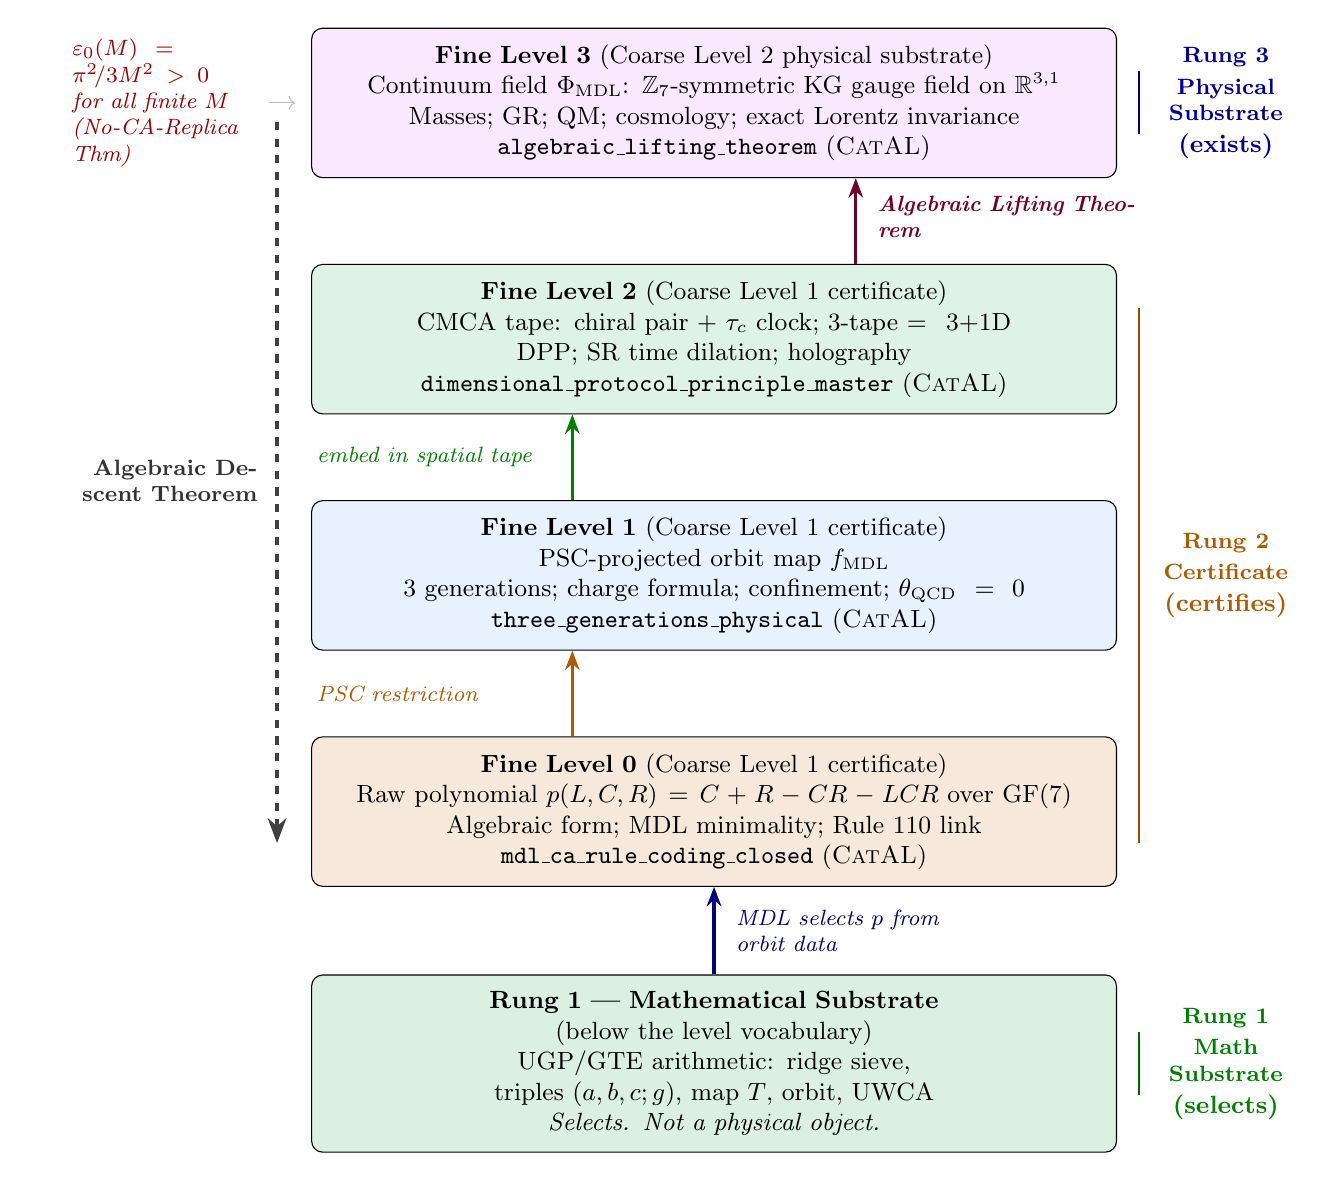
\begin{tikzpicture}[
  every node/.style={font=\small},
  box/.style={draw,rounded corners=4pt,minimum width=9.8cm,
              align=center,inner sep=6pt,font=\small},
  lbl/.style={font=\footnotesize\itshape,align=left,text width=3.0cm},
  rlbl/.style={font=\footnotesize\bfseries,align=center,text width=2.0cm},
  arrow/.style={-{Stealth[length=7pt]},very thick},
  darrow/.style={-{Stealth[length=7pt]},thick,dashed,gray!60},
  ]

  %─── Rung 1: Mathematical Substrate ────────────────────────────────────────
  \node[box,fill=rungmath!80,text=black,text width=9.8cm]
    (math) at (0,0)
    {\textbf{Rung~1 --- Mathematical Substrate}\\
     \normalfont\small (below the level vocabulary)\\
     UGP/GTE arithmetic: ridge sieve, triples $(a,b,c;g)$, map $T$, orbit, UWCA\\
     \textit{Selects. Not a physical object.}};

  %─── Level 0 ────────────────────────────────────────────────────────────────
  \node[box,fill=levzero!90,text=black,text width=9.8cm]
    (lev0) at (0, 3.2)
    {\textbf{Fine Level~0} (Coarse Level~1 certificate)\\
     \normalfont\small Raw polynomial $p(L,C,R)=C+R-CR-LCR$ over $\mathrm{GF}(7)$\\
     Algebraic form; MDL minimality; Rule~110 link\\
     \texttt{mdl\_ca\_rule\_coding\_closed} (\CatAL)};

  %─── Level 1 ────────────────────────────────────────────────────────────────
  \node[box,fill=levone!90,text=black,text width=9.8cm]
    (lev1) at (0, 6.2)
    {\textbf{Fine Level~1} (Coarse Level~1 certificate)\\
     \normalfont\small PSC-projected orbit map $f_{\rm MDL}$\\
     3 generations; charge formula; confinement; $\theta_{\rm QCD}=0$\\
     \texttt{three\_generations\_physical} (\CatAL)};

  %─── Level 2 ────────────────────────────────────────────────────────────────
  \node[box,fill=levtwo!90,text=black,text width=9.8cm]
    (lev2) at (0, 9.2)
    {\textbf{Fine Level~2} (Coarse Level~1 certificate)\\
     \normalfont\small CMCA tape: chiral pair + $\tau_c$ clock; 3-tape $= 3{+}1$D\\
     DPP; SR time dilation; holography\\
     \texttt{dimensional\_protocol\_principle\_master} (\CatAL)};

  %─── Rung 2 label ──────────────────────────────────────────────────────────
  \node[rlbl,text=orange!70!black]
    at (6.5, 6.2)
    {Rung~2\\[2pt] Certificate\\[2pt] \small(certifies)};

  %─── Rung 2 vertical bar ───────────────────────────────────────────────────
  \draw[orange!60!black,thick]
    (5.4, 2.8) -- (5.4, 9.6);

  %─── Level 3 ────────────────────────────────────────────────────────────────
  \node[box,fill=levthree!90,text=black,text width=9.8cm]
    (lev3) at (0, 12.2)
    {\textbf{Fine Level~3} (Coarse Level~2 physical substrate)\\
     \normalfont\small Continuum field $\Phi_{\rm MDL}$: $\mathbb{Z}_7$-symmetric KG gauge
     field on $\mathbb{R}^{3,1}$\\
     Masses; GR; QM; cosmology; exact Lorentz invariance\\
     \texttt{algebraic\_lifting\_theorem} (\CatAL)};

  %─── Rung 3 label ──────────────────────────────────────────────────────────
  \node[rlbl,text=blue!60!black]
    at (6.5, 12.2)
    {Rung~3\\[2pt] Physical\\Substrate\\[2pt] \small(exists)};

  \draw[blue!50!black,thick]
    (5.4, 11.8) -- (5.4, 12.6);

  %─── Rung 1 label ──────────────────────────────────────────────────────────
  \node[rlbl,text=green!50!black]
    at (6.5, 0)
    {Rung~1\\[2pt] Math\\Substrate\\[2pt] \small(selects)};

  \draw[green!40!black,thick]
    (5.4, -0.4) -- (5.4, 0.4);

  %─── MDL selection arrow (Rung 1 → Level 0) ────────────────────────────────
  \draw[arrow,blue!50!black]
    (math.north) -- node[right=4pt,lbl]
    {MDL selects $p$ from orbit data}
    (lev0.south);

  %─── Level 0 → 1 arrow ──────────────────────────────────────────────────────
  \draw[arrow,orange!70!black]
    ([xshift=-1.8cm]lev0.north) -- node[left=3pt,lbl]
    {PSC restriction}
    ([xshift=-1.8cm]lev1.south);

  %─── Level 1 → 2 arrow ──────────────────────────────────────────────────────
  \draw[arrow,green!50!black]
    ([xshift=-1.8cm]lev1.north) -- node[left=3pt,lbl]
    {embed in spatial tape}
    ([xshift=-1.8cm]lev2.south);

  %─── Lifting arrow (Level 2 → 3) ────────────────────────────────────────────
  \draw[arrow,purple!60!black]
    ([xshift=1.8cm]lev2.north) --
    node[pos=0.55,right=4pt,lbl,text=purple!60!black,text width=3.4cm]
    {\textbf{Algebraic Lifting Theorem}}
    ([xshift=1.8cm]lev3.south);

  %─── Descent arrow (outside left edge of Levels 0–3, Level 3 → Level 0) ────
  % Box is 9.8cm wide, half = 4.9cm; left edge of box at x = -4.9cm.
  % Arrow runs at x = -5.8cm, clearly outside the box.
  \draw[{Stealth[length=9pt]}-,very thick,gray!50!black,dashed]
    (-5.55, 2.8) --
    (-5.55, 12.0);
  % Label to the LEFT of the arrow
  \node[font=\footnotesize\bfseries,align=right,text=gray!40!black,text width=2.8cm]
    at (-7.2, 7.4)
    {Algebraic Descent Theorem};

  %─── No-CA-Replica annotation ───────────────────────────────────────────────
  \node[font=\footnotesize\itshape,align=left,text=red!60!black,
        text width=2.3cm]
    at (-7.0, 12.2)
    {$\varepsilon_0(M)=\pi^2\!/3M^2 > 0$
     for all finite $M$
     (No-CA-Replica Thm)};

  \draw[->,gray!50,thin]
    (-5.65, 12.2) -- ([xshift=-0.2cm]lev3.west);

\end{tikzpicture}
\end{center}

\bigskip
\noindent
\textbf{Reading the diagram:}
\begin{itemize}[itemsep=4pt]
  \item The \textbf{solid upward arrows} on the left show the derivation
    chain: the mathematical substrate (Rung~1) produces the polynomial
    (Level~0) via MDL selection; the polynomial is restricted to
    PSC-admissible inputs to give the orbit map (Level~1); the orbit map
    is embedded in a spatial tape (Level~2); and the Algebraic Lifting
    Theorem lifts the tape's discrete structure to the continuum field
    (Level~3).
  \item The \textbf{dashed downward arrow} on the right shows the Descent
    Theorem: the algebraic structure certified at Level~1--2 must be
    respected by any continuum model at any resolution.
  \item The \textbf{curly braces} on the right label the two ontological
    rungs.
    Rung~1 (Mathematical Substrate) is at the bottom; the level vocabulary
    starts above it.
    Levels~0--2 are all on Rung~2 (Certificate).
    Level~3 alone is on Rung~3 (Physical Substrate).
  \item The \textbf{No-CA-Replica} annotation explains why Level~2 cannot
    be promoted to Level~3 by itself: any finite-resolution CA has a
    non-zero Lorentz error.
\end{itemize}

%═══════════════════════════════════════════════════════════════════════════════
\section{Summary}
\label{sec:summary}
%═══════════════════════════════════════════════════════════════════════════════

\begin{tcolorbox}[colback=boxblue,colframe=blue!40!black,
  title=The key things to remember]
\begin{enumerate}[itemsep=8pt]
  \item \textbf{The coarse two-level scheme} (used in most papers):
    Level~1 = algebraic certificate (discrete, machine-certifiable);
    Level~2 = physical substrate ($\PhiMDL$, continuum, exists).

  \item \textbf{The fine four-level scheme} (used in detailed derivations):
    Level~0 (raw polynomial) $\to$ Level~1 ($\fMDL$ orbit)
    $\to$ Level~2 (CMCA tape) $\to$ Level~3 ($\PhiMDL$ field).
    In the coarse scheme, Levels~0--2 all collapse to ``Level~1 certificate.''

  \item \textbf{The ontological ladder} has three rungs:
    Mathematical Substrate (selects, below the level vocabulary),
    Certificate (certifies, = fine Levels~0--2),
    Physical Substrate (exists, = fine Level~3).
    Levels grade \emph{resolution}; rungs grade \emph{role}.

  \item \textbf{The Algebraic Lifting Theorem}
    (\lean{algebraic\_lifting\_theorem}, \CatAL, zero sorry):
    every property certified at the discrete Level~1 must exist in the
    continuum Level~3 field.
    This is why proving a theorem about the CA is proving a theorem
    about particle physics.

  \item \textbf{The Algebraic Descent Theorem}
    (\lean{algebraic\_descent\_theorem}, \CatAL, zero sorry):
    every $F_{21}$ conservation law certified at the discrete level
    holds in any continuum realization at any resolution $M \geq 1$.
    The algebraic facts are $M$-independent.

  \item \textbf{The No-CA-Replica Theorem}
    (\lean{no\_finite\_ca\_exact\_lorentz\_replica}, \CatAL, zero sorry):
    no finite-resolution CA achieves exact Lorentz invariance.
    Only $\PhiMDL$ (the $M \to \infty$ continuum limit) achieves
    $\varepsilon_0 = 0$ exactly.
    The CA is not the universe; it is the universe's proof engine.

  \item \textbf{Level framing in papers:} every result carries a level label.
    Level~0--2 results are in principle machine-verifiable (\CatAL).
    Level~3 results additionally require the Lifting Theorem (\CatAD\ or above).
\end{enumerate}
\end{tcolorbox}

\bigskip\noindent
The full derivation chain is documented across the GTE paper series (P00--P51)
and machine-certified in over 300 Lean~4 modules (zero sorry, zero custom
axioms), all publicly available at \url{https://zenodo.org/records/20560550}
and \url{https://novaspivack.com/research}.

\section*{Further Reading}
\begin{tcolorbox}[colback=orange!8,colframe=orange!50!black,
  title=\textbf{Primary Sources}]
The results in this tutorial are derived and certified in the following
papers, all available open-access on Zenodo and at
\href{https://novaspivack.com/research}{novaspivack.com/research}:
\begin{itemize}[itemsep=4pt]
  \item \textbf{P48 --- The Complete GTE Framework} (main synthesis monograph;
    Chapter~4 Mathematical Substrate, Chapter~6 One Field --- Lifting and
    Descent, four-level architecture box in Chapter~6):\\
    \href{https://doi.org/10.5281/zenodo.20560550}{doi.org/10.5281/zenodo.20560550}
  \item \textbf{P41 --- The Three-Layer Chiral Minkowski CA} (Level~2 CMCA
    architecture):\\
    \href{https://doi.org/10.5281/zenodo.20417572}{doi.org/10.5281/zenodo.20417572}
  \item \textbf{P43 --- The Complete $\Phi_{\rm MDL}$ Framework} (no-CA-replica
    theorem; Lifting and Descent theorems):\\
    \href{https://doi.org/10.5281/zenodo.20417578}{doi.org/10.5281/zenodo.20417578}
  \item \textbf{P45 --- The Three-Tape CMCA} (Dimensional Protocol Principle;
    3+1D architecture):\\
    \href{https://doi.org/10.5281/zenodo.20465805}{doi.org/10.5281/zenodo.20465805}
  \item \textbf{P46 --- The GTE Polynomial as UFT} (five simultaneous physical
    roles; Level framing):\\
    \href{https://doi.org/10.5281/zenodo.20465809}{doi.org/10.5281/zenodo.20465809}
\end{itemize}
Lean~4 machine proofs:
\href{https://github.com/novaspivack/ugp-lean}{github.com/novaspivack/ugp-lean}
\end{tcolorbox}

\bibliography{../../papers/bib/Spivack_Papers_Bibliography}
\end{document}
